\documentclass[12pt,letterpaper]{article}
\usepackage[utf8]{inputenc}
\usepackage[spanish]{babel}
\usepackage{graphicx}
\usepackage[left=2cm,right=2cm,top=2cm,bottom=2cm]{geometry}
\usepackage{graphicx} % figuras
% \usepackage{subfigure} % subfiguras
\usepackage{float} % para usar [H]
\usepackage{amsmath}
%\usepackage{txfonts}
\usepackage{stackrel} 
\usepackage{multirow}
\usepackage{enumerate} % enumerados

\usepackage{hyperref}
\renewcommand{\labelitemi}{$-$}
\renewcommand{\labelitemii}{$\cdot$}
% \author{}
% \title{Caratula}
\begin{document}

% Fancy Header and Footer
% \usepackage{fancyhdr}
% \pagestyle{fancy}
% \cfoot{}
% \rfoot{\thepage}
%

% \usepackage[hidelinks]{hyperref} % CREA HYPERVINCULOS EN INDICE

% \author{}
\title{Caratula}

\begin{titlepage}
\begin{center}
\begin{figure}[htb]
\begin{center}

\includegraphics[width=3.5cm]{./img/logo}
\end{center}
\end{figure}

\vspace*{0.15in}
\begin{Large}
\textbf{UNIVERSIDAD PRIVADA DE TACNA}\\
\end{Large}

\vspace*{0.1in}
\begin{Large}
\textbf{FACULTAD DE INGENIERIA} \\
\end{Large}

\vspace*{0.1in}
\begin{Large}
\textbf{ESCUELA PROFESIONAL DE INGENIERIA DE SISTEMAS} \\
\end{Large}

\vspace*{0.5in}
\begin{Large}
\textbf{TITULO:}\\
\end{Large}

\vspace*{0.1in}
\begin{Large}
INFORME DE LABORATORIO Nº 02\\
\end{Large}

\vspace*{0.3in}
\begin{Large}
\textbf{CURSO:} \\
\end{Large}

\vspace*{0.1in}
\begin{large}
INTELIGENCIA DE NEGOCIOS\\
\end{large}

\vspace*{0.3in}
\begin{Large}
\textbf{DOCENTE:} \\
\end{Large}

\vspace*{0.1in}
\begin{large}
Ing. Patrick José Cuadros Quiroga\\
\end{large}

\vspace*{0.2in}
\vspace*{0.1in}
\begin{large}
Integrantes: \\
\begin{flushleft}

Cancino Tapia, Luis Antonio 		\hfill	(2015052383) \\

\end{flushleft}
\end{large}
\vspace*{0.1in}
\begin{large}
Tacna - Perú\\
\end{large}
\vspace*{0.1in}
\begin{large}
2021\\
\end{large}

\end{center}

\end{titlepage}

\include{Secciones/articulo}
%%%%%%%%%%%%%%%%%%%%%%%%%%%%%%%%%%%%%%%%%%%%%%%%%%%%%%%%%
\vspace*{0.1in}

\begin{LARGE}
    \begin{center}
        \textbf{INFORME DE LABORATORIO Nº 01} \\
    \end{center}
\end{LARGE}
\vspace*{0.1in}

\section{DESARROLLO}
\begin{enumerate}
    \item Crea una nueva aplicación.
    \begin{itemize}
        \item Inicie Qlik Sense.
        \item Cree una nueva aplicación.
        \item Nombre la aplicación: "My Sales Analysis".
        \item Crear y abrir la aplicación.
    \end{itemize}
        \begin{center}
            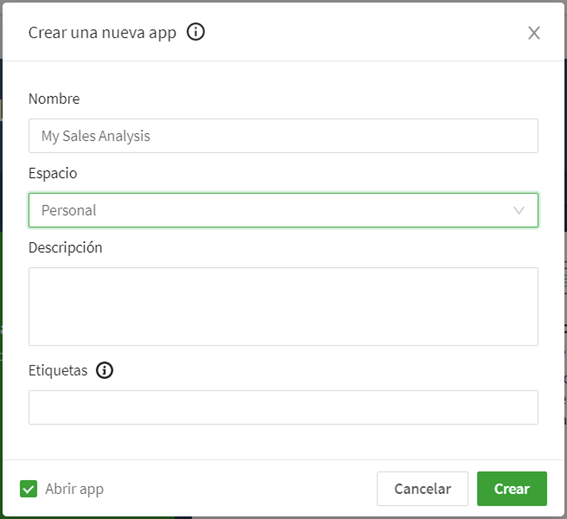
\includegraphics[width=10cm]{./img/image1.png} 
        \end{center}
    \item Cargar datos.
    \begin{itemize}
        \item Utilice el mosaico Agregar datos de archivos y otras fuentes para agregar el Datos de Excel a la aplicación (desde el archivo ExerciseData.xlsx).
        \item Cargue todos los campos de la hoja de cálculo, haciendo clic en Agregar datos botón.
    \end{itemize}

    \item Revisar datos.
    \begin{itemize}
        \item Utilice el menú de acceso rápido para navegar a la vista Administrador de datos, en para obtener más información sobre esta tabla.
        \item Abra la vista del editor de tablas del administrador de datos haciendo clic en el icono a lo largo de la parte inferior de la vista.
        \item Haga clic en los campos indicados y vea la tarjeta de resumen para responder a la siguientes preguntas:
        \begin{itemize}
            \item ¿Cuántos valores de Country distintos están presentes en esta tabla? (Answer = 21)
            \item ¿Cuántos valores distintos hay para Product Category campo? (Answer = 8)
            \item ¿Cuántos valores distintos hay para el campo Product? (Answer = 74)
            \item ¿Cuántos valores distintos hay para el campo Source? (Answer = 2); ¿Cuáles son esos dos valores? (Answer = Existente Cuentas y cuentas nuevas)
        \end{itemize}
    \end{itemize}

    \item Desarrolle una hoja con el "Asesor de conocimientos".\\
    \begin{itemize}
        \item Utilice el submenú de navegación de acceso rápido en Analizar> Hoja para seleccionar Insights, haga clic en el botón para generar conocimientos, basados en todo el modelo de datos.
        \item Ubique el mapa en la lista de gráficos propuestos y Agregar a hoja> Mi nueva hoja.
        \item Utilice el panel de la izquierda para seleccionar (casillas marcadas) los campos: Producto y Precio unitario.
        \begin{itemize}
            \item Busque el gráfico de barras titulado: suma (PrecioUnitario) por Producto y Agregar a la hoja> Mi nueva hoja.
            \item Borre los campos ().
        \end{itemize}
        \item Escriba lo siguiente en el campo "Háganos una pregunta": ¿Qué país tiene la mayor cantidad? (y enviar pregunta).
        \begin{itemize}
            \item Busque el gráfico de barras titulado: suma (Cantidad) por país y Agregar a la hoja> Mi nueva hoja.
        \end{itemize}
        \item Utilice el submenú de navegación de acceso rápido en Analizar> Perspectivas para seleccionar Hoja y evaluar la hoja que ha creado. Debería aparecer como ve a continuación:
        \begin{center}
            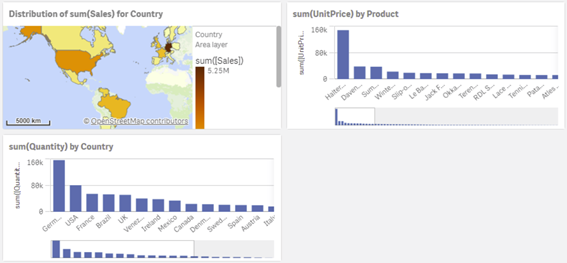
\includegraphics[width=15cm]{./img/image2.png} 
        \end{center}
        \item Cambie la hoja al modo de edición () y use el panel de propiedades para cambiar el título de la hoja de "Mi nueva hoja" a "Mis ideas".
        \begin{itemize}
            \item SUGERENCIA: Si está oculto, muestre el panel de propiedades (usando el icono en la esquina inferior derecha) y no active ninguno de los gráficos en la hoja. Esto garantizará que las propiedades de la hoja estén disponibles para su edición, incluido el título de la hoja.
        \end{itemize}
    \end{itemize}
    \item Desarrolle una hoja utilizando ``Ayuda para sugerencias de gráficos"\\
    \begin{itemize}
        \item Utilice el menú desplegable de hojas para crear una nueva hoja.
        \begin{itemize}
            \item Titular la hoja: “Mis sugerencias”.
        \end{itemize}
        \item En el modo Editar hoja, use la sección Campos del panel de activos, arrastre y suelte el campo Ventas en el área de visualización.
        \begin{itemize}
            \item Resultados de tipo gráfico de KPI, que muestra la suma de los valores de ventas para todo el modelo de datos.
            \item Además, el interruptor de sugerencias de gráficos en la parte superior del panel de propiedades está configurado en ``activado".\\
        \end{itemize}
        \begin{center}
            \includegraphics[width=8cm]{./img/image3.png} 
            \includegraphics[width=8cm]{./img/image4.png}
        \end{center}
        \item Arrastre y suelte el campo País en el gráfico de KPI, asegurándose de que la imagen "fantasma" cubra todo el gráfico.
        \begin{itemize}
            \item Se obtiene un tipo de gráfico de mapa y el color en el mapa relaciona la suma de los valores de ventas en cada país.
        \end{itemize}
        \begin{center}
            \includegraphics[width=13cm]{./img/image5.png} 
        \end{center}
    \end{itemize}
    \item Desarrolle una hoja usando "Ayuda para sugerencias de gráficos" (cont.)\\
    \begin{itemize}
        \item Expanda el campo OrderDate en el panel de activos para exponer agrupaciones de fechas derivadas.
        \begin{itemize}
            \item Arrastre y suelte la agrupación YearMonth en un espacio vacío en el área de visualización.
            \item Una tabla de resultados tipo gráfico.
        \end{itemize}
        \item Arrastre y suelte el campo Ventas para cubrir toda la tabla que actualmente muestra los valores de año y mes para pedidos.
        \begin{itemize}
            \item Resultados de un gráfico de líneas, debido al hecho de que se ha proporcionado una dimensión de fecha y un campo de valores de medida a esta visualización.
        \end{itemize}
        \begin{center}
            \includegraphics[width=9cm]{./img/image6.png} 
        \end{center}
        \item Arrastre y suelte el campo Cantidad para cubrir todo el gráfico de líneas.
        \begin{itemize}
            \item Se obtiene un gráfico combinado, debido a que se proporcionaron una dimensión y múltiples medidas (que ocupan diferentes rangos).
            \item Haga clic en el botón Finalizar edición y use el control deslizante de zoom del minigráfico, debajo del gráfico combinado, para examinar los valores mes-año más recientes.
        \end{itemize}
        \begin{center}
            \includegraphics[width=15cm]{./img/image7.png} 
        \end{center}
    \end{itemize}
    \item Pruebe un tipo de gráfico alternativo sugerido\\
    \begin{itemize}
        \item Vuelva al modo Editar hoja y considere sugerencias de gráficos alternativos.
        \begin{itemize}
            \item Cambie del gráfico combinado recomendado a un gráfico de líneas.
            \begin{center}
                \includegraphics[width=10cm]{./img/image8.png} 
            \end{center}
        \end{itemize}
    \end{itemize}
    \item Cambie el interruptor de sugerencias de gráficos de ''activado" a "desactivado"
    \begin{itemize}
        \item Tenga en cuenta que el panel de propiedades de los gráficos configurados con ayuda presenta solo opciones de configuración limitadas para que las ajuste.
        \item Nos gustaría ajustar la combinación de colores aplicada a las formas de los países en el gráfico de mapa, así que cambie el interruptor de sugerencias de gráficos a "desactivado".
        \begin{itemize}
            \item Abra la sección Capas del panel de propiedades y haga clic en la capa Área del país.
            \begin{itemize}
                \item Abra la sección Colores y localice las opciones de Esquema de colores.
                \begin{itemize}
                    \item Cambie el esquema de color de degradado secuencial a degradado divergente.
                    \item Marque la casilla de verificación Invertir colores.
                \end{itemize}
            \end{itemize}
        \end{itemize}
        \item El mapa resultante debería aparecer como se ve a continuación.
        \begin{center}
            \includegraphics[width=12cm]{./img/image9.png} 
        \end{center}
    \end{itemize}
    \item Desarrollar una hoja sin ayuda
    \begin{itemize}
        \item Cree una nueva hoja en la aplicación, titulada "Mis gráficos personalizados".
        \item Arrastre y suelte objetos desde la sección Gráficos () del panel de activos al área de visualización y cambie el tamaño de cada uno para completar una hoja con un gráfico de barras, una tabla, un gráfico circular, un KPI, un panel de filtros y un área de texto e imagen organizada dentro el espacio de visualización como se muestra a continuación:
        \begin{center}
            \includegraphics[width=10cm]{./img/image10.png} 
        \end{center}
    \end{itemize}
    \item Desarrolle una hoja sin ayuda (cont.)
    \begin{itemize}
        \item Configuración del gráfico de barras:
        \begin{itemize}
            \item Dimensión = Categoría de producto
            \item Medida = Ventas, agregadas con una suma: Suma (Ventas)
            \item Agregue un título al gráfico que diga: "Ventas totales por categoría de producto".
        \end{itemize}
        \item Configuración de la mesa:
        \begin{itemize}
            \item Dimensión = Producto
            \item Desde la sección Campos () del panel de activos, arrastre y suelte el campo Ventas para cubrir toda la tabla.
            \begin{itemize}
                \item Agregar como medida, agregar con una Suma: Suma (Ventas)
                \item Utilice la sección Datos del panel de propiedades para expandir la subsección de medida Suma de ventas y formatee la suma de valores de ventas de la siguiente manera:
                \begin{itemize}
                    \item Formato de número = Número
                    \item Formateo = simple; 1.000
                \end{itemize}
            \end{itemize}
        \end{itemize}
        \item Configuración de gráfico circular:
        \begin{itemize}
            \item Dimensión (Slice) = Fuente
            \item Medida (ángulo) = Ventas, agregadas con una Suma: Suma (Ventas)
            \item Agregue un título al gráfico que diga: "Ventas para cuentas nuevas frente a cuentas existentes".
        \end{itemize}   
        \item Configuración de KPI:
        \begin{itemize}
            \item Medida = Ventas, agregadas con una Suma: Suma (Ventas)
        \end{itemize} 
        \item Configuración del panel de filtro:
        \begin{itemize}    
            \item Dimensión = OrderDate.Year (SUGERENCIA: busque OrderDate y de la lista resultante: seleccione la agrupación de fechas derivada que agrupa las fechas por año).
            \begin{itemize}      
                \item Expanda la subsección de dimensión resultante y edite el Título a: “Año”.
            \end{itemize} 
        \end{itemize} 
        \item Configuración de texto e imagen:
        \begin{itemize}  
            \item Ingrese el texto: "Seleccione un año de interés para limitar los datos".
        \end{itemize} 
    \end{itemize}  
    \item Desarrolle una hoja sin ayuda (cont.)
    \begin{itemize}  
        \item La hoja que configuró debería aparecer como se ve a continuación:
        \begin{center}
            \includegraphics[width=10cm]{./img/image11.png} 
        \end{center}
    \end{itemize} 
    \item Analizar una hoja
    \begin{itemize}  
        \item Seleccione el año 2013, tome una instantánea del gráfico circular, anote con “2013”.
        \begin{itemize}  
            \item Borrar la selección.
        \end{itemize} 
        \item Seleccione el año 2015 y tome una instantánea del gráfico circular, anote con “2015”.
        \begin{itemize}  
            \item Borrar la selección.
        \end{itemize} 
        \item Haga clic para realizar las siguientes tres selecciones ...
        \begin{itemize}  
            \item Seleccione la barra Traje de baño en el gráfico de barras y confirme la selección.
            \item Seleccione el año 2017 en el panel de filtros y confirme la selección.
            \item Seleccione la sección Cuentas nuevas en el gráfico circular y confirme la selección.
            \item ...luego crea un nuevo marcador:
            \begin{itemize}  
                \item Nombre el marcador = "Nuevas cuentas, trajes de baño, 2017"
            \end{itemize} 
        \end{itemize} 
        \item Borre todas las selecciones y cree un segundo marcador que limite las visualizaciones a los datos de 2014.
        \begin{itemize}  
            \item Nombre el marcador = "pedidos de 2014"
        \end{itemize}
        \item Utilice los dos marcadores para alternar entre estos diferentes estados de los datos seleccionados.
    \end{itemize} 
    \item Contar una historia
    \begin{itemize}  
        \item Utilice el menú de acceso rápido para navegar a la vista Narración.
        \item Utilice la biblioteca de instantáneas () para agregar las dos instantáneas que tomó a la diapositiva en blanco.
        \item Utilice la biblioteca de texto () para agregar una etiqueta para 2013 (al gráfico circular con la porción más pequeña de Cuentas Nuevas).
        \item Agregue otra etiqueta para 2015 (al gráfico circular con la porción de Cuentas Nuevas más grande).
        \item Utilice la biblioteca de hojas () para agregar la hoja titulada Mis sugerencias a una diapositiva de la historia.
        \item Reproducir la historia (). Haga clic en diferentes aspectos visuales de su hoja de datos en vivo (como formas de países individuales) para ver que es una diapositiva interactiva.
        \begin{center}
            \includegraphics[width=12cm]{./img/image12.png}
            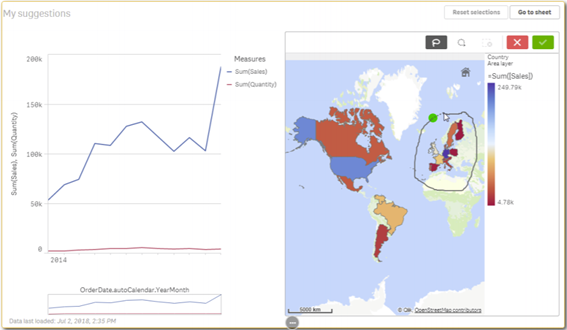
\includegraphics[width=12cm]{./img/image13.png}  
        \end{center}
    \end{itemize}
    
\section{CONCLUSIONES}
\begin{itemize}
    \item Continúe analizando los datos de este ejemplo agregando más hojas y más diapositivas a su historia. Revise el modelo de datos, según sea necesario, para comprender la naturaleza de los campos en esta sencilla tabla a medida que desarrolla y realiza su análisis.\\
\end{itemize}
\end{enumerate}

%%%%%%%%%%%%%%%%%%%%%%%%%%%%%%%%%%%%%%%%%%%%%%%%%%%%%%%%%
\end{document}






